\begin{enumerate}[label=\thesubsection.\arabic*, ref=\thesubsection.\theenumi]
\item
Find the domain of the function $f\brak{x} = \cos^{-1}x + \sin x$.
\hfill (12, 2025)
% TODO: add options (A)-(D) from the paper; the answer is option (C)

\solution
$\cos^{-1}x$ is defined only for $-1 \le x \le 1$, and $\sin x$ is defined for every real $x$. The domain of the sum is the intersection of the two domains:
\begin{align}
	\text{Domain}\brak{f} = \sbrak{-1,1} \quad \brak{\text{Option C}}
\end{align}
The program scans $x$ over $\sbrak{-3,3}$ and treats the points where \texttt{acos(x)+sin(x)} is not a number as outside the domain. The following code verifies the solution
\begin{lstlisting}[frame=single, basicstyle=\rmfamily, escapeinside={(*@}{@*)}]
(*@\makebox[\dimexpr\linewidth-2\fboxsep-2\fboxrule\relax][c]{12/codes/2.py}@*)
\end{lstlisting}

\item
The number of all possible matrices of order $3 \times 3$ with each entry $2$ or $3$ is
\hfill (12, 2025)
% TODO: add options (A)-(D) from the paper; the answer is option (B)

\solution
Each of the $9$ entries can independently be $2$ or $3$. By the multiplication principle,
\begin{align}
	N = 2^9 = 512 \quad \brak{\text{Option B}}
\end{align}
The following code generates every $3\times3$ matrix with entries $2$ or $3$ and counts them in the loop
\begin{lstlisting}[frame=single, basicstyle=\rmfamily, escapeinside={(*@}{@*)}]
(*@\makebox[\dimexpr\linewidth-2\fboxsep-2\fboxrule\relax][c]{12/codes/3.py}@*)
\end{lstlisting}

\item
The matrix $\vec{A} = \myvec{3 & 0 & 0 \\ 0 & 2 & 0 \\ 0 & 0 & 5}$ is a
\hfill (12, 2025)
\begin{enumerate}
	\begin{multicols}{4}
    \item scalar matrix
    \item identity matrix
    \item null matrix
    \item symmetric matrix
	\end{multicols}
\end{enumerate}

\solution
(theory only) A matrix is symmetric if $\vec{A}^{\top} = \vec{A}$. For a diagonal matrix the transpose leaves every entry unchanged,
\begin{align}
	\vec{A}^{\top} = \myvec{3 & 0 & 0 \\ 0 & 2 & 0 \\ 0 & 0 & 5} = \vec{A}
\end{align}
The diagonal entries are not all equal, so $\vec{A}$ is not a scalar matrix; it is neither the identity nor the null matrix. Hence $\vec{A}$ is a symmetric matrix $\brak{\text{Option D}}$.

\item
If $\vec{A}$ and $\vec{B}$ are square matrices of order $3$ with $\abs{\vec{A}} = 3$ and $\abs{\vec{B}} = 5$, then $\abs{2\vec{A}\vec{B}}$ is
\hfill (12, 2025)
% TODO: add options (A)-(D) from the paper; the answer is option (B)

\solution
Following matgeo, the characteristic polynomial of a square matrix $\vec{M}$ is $f\brak{\lambda} = \abs{\vec{M} - \lambda\vec{I}}$, so
\begin{align}
	\abs{\vec{M}} = f\brak{0} = \lambda_1\lambda_2\lambda_3
\end{align}
where $\lambda_i$ are the eigenvalues. The eigenvalues of $2\vec{A}\vec{B}$ are not those of $\vec{A}$ and $\vec{B}$ separately, so we use $\abs{k\vec{A}} = k^n\abs{\vec{A}}$ and $\abs{\vec{A}\vec{B}} = \abs{\vec{A}}\abs{\vec{B}}$. With $n = 3$,
\begin{align}
	\abs{2\vec{A}\vec{B}} = 2^3\abs{\vec{A}}\abs{\vec{B}} = 8\brak{3}\brak{5} = 120 \quad \brak{\text{Option B}}
\end{align}
To check this numerically, take $\vec{A} = \myvec{1 & 1 & 0 \\ 0 & 1 & 1 \\ 1 & 0 & 2}$ with $\abs{\vec{A}} = 3$ and $\vec{B} = \myvec{1 & -1 & -1 \\ -1 & 1 & 0 \\ 2 & 3 & 1}$ with $\abs{\vec{B}} = 5$. The program obtains the characteristic polynomial of $\vec{M} = 2\vec{A}\vec{B}$ from \texttt{numpy.poly}, which returns $\det\brak{\lambda\vec{I} - \vec{M}}$, and reads $\abs{\vec{M}} = \brak{-1}^3 c_0$ from its constant term $c_0$. The following code verifies the solution
\begin{lstlisting}[frame=single, basicstyle=\rmfamily, escapeinside={(*@}{@*)}]
(*@\makebox[\dimexpr\linewidth-2\fboxsep-2\fboxrule\relax][c]{12/codes/5.py}@*)
\end{lstlisting}

\item
If $\vec{A}$ is a square matrix of order $3$ with $\abs{\vec{A}} = 5$, then $\abs{\text{adj}\,\vec{A}}$ is
\hfill (12, 2025)
% TODO: add options (A)-(D) from the paper; the answer is option (C)

\solution
For a square matrix of order $3$,
\begin{align}
	\vec{A}\,\text{adj}\,\vec{A} = \abs{\vec{A}}\vec{I}
\end{align}
Taking the determinant of both sides and using $\abs{k\vec{I}} = k^3$ for order $3$,
\begin{align}
	\abs{\vec{A}}\abs{\text{adj}\,\vec{A}} = \abs{\vec{A}}^3
	\implies \abs{\text{adj}\,\vec{A}} = \abs{\vec{A}}^2 = 5^2 = 25 \quad \brak{\text{Option C}}
\end{align}
since $\abs{\vec{A}} = 5 \neq 0$. The program builds $\text{adj}\,\vec{A}$ from the cofactors of an example matrix with $\abs{\vec{A}} = 5$ and checks that $\vec{A}\,\text{adj}\,\vec{A} = 5\vec{I}$ and $\abs{\text{adj}\,\vec{A}} = 25$. The following code verifies the solution
\begin{lstlisting}[frame=single, basicstyle=\rmfamily, escapeinside={(*@}{@*)}]
(*@\makebox[\dimexpr\linewidth-2\fboxsep-2\fboxrule\relax][c]{12/codes/6.py}@*)
\end{lstlisting}

\item
The function $f\brak{x} = 2x - \sin x$, $x \in \mathbb{R}$, is
\hfill (12, 2025)
\begin{enumerate}
	\begin{multicols}{2}
    \item strictly decreasing on $\mathbb{R}$
    \item strictly increasing on $\mathbb{R}$
    \item neither increasing nor decreasing on $\mathbb{R}$
    \item decreasing on $\brak{-\infty,0}$ and increasing on $\brak{0,\infty}$
	\end{multicols}
\end{enumerate}
% TODO: confirm the wording of options (A), (C), (D) against the paper

\solution
Differentiating,
\begin{align}
	f^{\prime}\brak{x} = 2 - \cos x
\end{align}
Since $-1 \le \cos x \le 1$,
\begin{align}
	1 \le f^{\prime}\brak{x} \le 3 \implies f^{\prime}\brak{x} > 0 \quad \forall x \in \mathbb{R}
\end{align}
A differentiable function with a strictly positive derivative is strictly increasing, so $f$ is strictly increasing on $\mathbb{R}$ $\brak{\text{Option B}}$. The program checks that $f^{\prime}\brak{x} > 0$ at every point of a fine grid. The following code verifies the solution
\begin{lstlisting}[frame=single, basicstyle=\rmfamily, escapeinside={(*@}{@*)}]
(*@\makebox[\dimexpr\linewidth-2\fboxsep-2\fboxrule\relax][c]{12/codes/11.py}@*)
\end{lstlisting}
The following code generates \figref{fig:CBSE12-q11}.
\begin{lstlisting}[frame=single, basicstyle=\rmfamily, escapeinside={(*@}{@*)}]
(*@\makebox[\dimexpr\linewidth-2\fboxsep-2\fboxrule\relax][c]{12/codes/11plot.py}@*)
\end{lstlisting}
\begin{figure}[H]
	\centering
	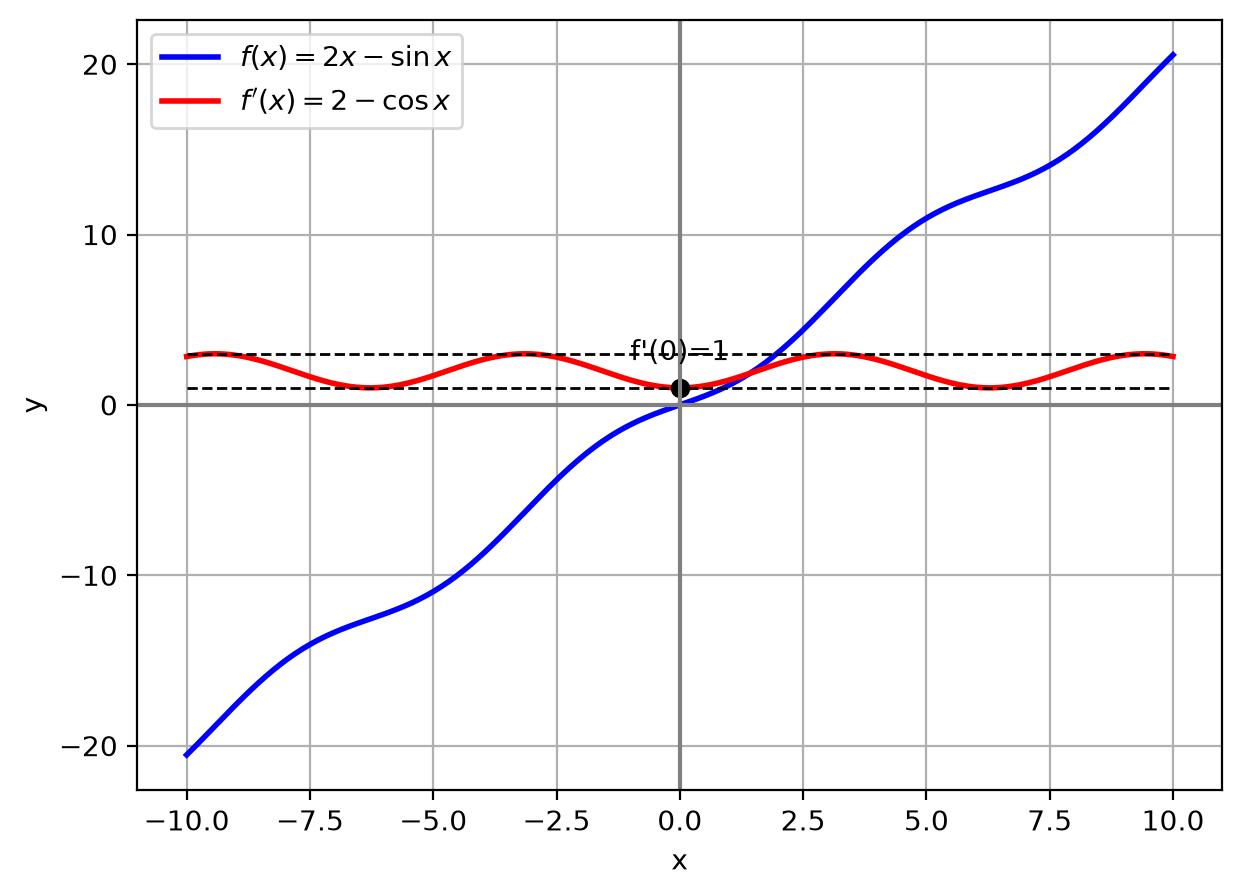
\includegraphics[width=0.7\linewidth]{figs/c12_q11.png}
	\caption{$f\brak{x}$ and $f^{\prime}\brak{x}$ with $1 \le f^{\prime}\brak{x} \le 3$}
	\label{fig:CBSE12-q11}
\end{figure}

\item
Which of the following statements is correct?
\hfill (12, 2025)
\begin{enumerate}[label=(\Alph*)]
	\item $\displaystyle\int_a^b f\brak{x}\,dx = \int_a^b f\brak{a+b-x}\,dx$
	\item $\displaystyle\int_{-a}^{a} f\brak{x}\,dx = 0$ if $f$ is even
	\item $\displaystyle\int_{-a}^{a} f\brak{x}\,dx = 2\int_0^a f\brak{x}\,dx$ if $f$ is odd
	\item $\displaystyle\int_0^{2a} f\brak{x}\,dx = \int_0^a f\brak{x}\,dx - \int_0^a f\brak{2a+x}\,dx$
\end{enumerate}
% TODO: confirm the exact wording of options (B)-(D) against the paper

\solution
\textbf{(A)} Put $u = a+b-x$, $du = -dx$. When $x = a$, $u = b$ and when $x = b$, $u = a$, so
\begin{align}
	\int_a^b f\brak{a+b-x}\,dx = \int_b^a f\brak{u}\brak{-du} = \int_a^b f\brak{u}\,du
\end{align}
(A) is true.

\textbf{(B)} For an even function $\int_{-a}^{a} f = 2\int_0^a f$. With $f\brak{x} = x^2$, $\int_{-1}^{1}x^2\,dx = \frac{2}{3} \neq 0$. False.

\textbf{(C)} For an odd function $\int_{-a}^{a} f = 0$. With $f\brak{x} = x$, the left side is $0$ and the right side is $1$. False.

\textbf{(D)} The correct splitting is $\int_0^{2a} f = \int_0^a f + \int_0^a f\brak{a+x}\,dx$. With $f\brak{x}=x$, $a=1$, the left side is $2$ and the right side is $-2$. False.

Hence the correct statement is (A). The program evaluates each statement as a boolean on sample functions: (A) must hold for every test function, while (B) and (C) are implications of the form (``$f$ is even'' $\implies$ identity), which are false as soon as a test function satisfies the premise but violates the conclusion. The following code verifies the solution
\begin{lstlisting}[frame=single, basicstyle=\rmfamily, escapeinside={(*@}{@*)}]
(*@\makebox[\dimexpr\linewidth-2\fboxsep-2\fboxrule\relax][c]{12/codes/13.py}@*)
\end{lstlisting}

\item
If $\vec{a}$ and $\vec{b}$ are two vectors such that $\abs{\vec{a}+\vec{b}} = \abs{\vec{a}-\vec{b}}$, then $\vec{a}$ and $\vec{b}$ are
\hfill (12, 2025)
% TODO: add options (A)-(D) from the paper; the answer is option (A)

\solution
(theory only) Squaring both sides and using $\abs{\vec{x}}^2 = \vec{x}^{\top}\vec{x}$,
\begin{align}
	\abs{\vec{a}}^2 + 2\vec{a}^{\top}\vec{b} + \abs{\vec{b}}^2 &= \abs{\vec{a}}^2 - 2\vec{a}^{\top}\vec{b} + \abs{\vec{b}}^2
	\\
	\implies 4\vec{a}^{\top}\vec{b} &= 0
\end{align}
Hence $\vec{a}$ and $\vec{b}$ are orthogonal $\brak{\text{Option A}}$; the zero vector is the trivial case.

\item
If $\pr{A} = \frac{1}{7}$, $\pr{B} = \frac{5}{7}$ and $\pr{A \cap B} = \frac{4}{7}$, find $\pr{A^{\prime} \mid B}$.
\hfill (12, 2025)
% TODO: these values are as transcribed in the chat; P(A and B) > P(A), so please
% re-check the probabilities against the paper before submitting.

\solution
Let $X$ take the values $0$, $1$, $2$ for the outcomes $A\cap B$, $A^{\prime}\cap B$ and $B^{\prime}$ respectively. From $\pr{B} = \frac{5}{7}$ and $\pr{A\cap B} = \frac{4}{7}$,
\begin{table}[H]
	\centering
	\begin{tabular}{|c|c|c|c|}
		\hline
		$x$ & $0$ $\brak{A\cap B}$ & $1$ $\brak{A^{\prime}\cap B}$ & $2$ $\brak{B^{\prime}}$ \\ \hline
		$p_X\brak{x}$ & $\frac{4}{7}$ & $\frac{5}{7} - \frac{4}{7} = \frac{1}{7}$ & $1 - \frac{5}{7} = \frac{2}{7}$ \\ \hline
	\end{tabular}
	\caption{pmf of $X$}
	\label{tab:CBSE12-q17}
\end{table}
Then $\pr{B} = p_X\brak{0} + p_X\brak{1} = \frac{5}{7}$ and $\pr{A^{\prime}\cap B} = p_X\brak{1} = \frac{1}{7}$, so
\begin{align}
	\pr{A^{\prime}\mid B} = \frac{\pr{A^{\prime}\cap B}}{\pr{B}} = \frac{1/7}{5/7} = \frac{1}{5}
\end{align}
The values as printed are not consistent with each other, because an intersection cannot be more probable than $A$ alone ($\frac{4}{7} > \frac{1}{7}$); the answer above uses only $\pr{B}$ and $\pr{A\cap B}$. The following program simulates $10^6$ draws from this pmf
\begin{lstlisting}[frame=single, basicstyle=\rmfamily, escapeinside={(*@}{@*)}]
(*@\makebox[\dimexpr\linewidth-2\fboxsep-2\fboxrule\relax][c]{12/codes/17.c}@*)
\end{lstlisting}
The following code makes a stem plot of the simulated relative frequencies and the pmf, see \figref{fig:CBSE12-q17}.
\begin{lstlisting}[frame=single, basicstyle=\rmfamily, escapeinside={(*@}{@*)}]
(*@\makebox[\dimexpr\linewidth-2\fboxsep-2\fboxrule\relax][c]{12/codes/17plot.py}@*)
\end{lstlisting}
\begin{figure}[H]
	\centering
	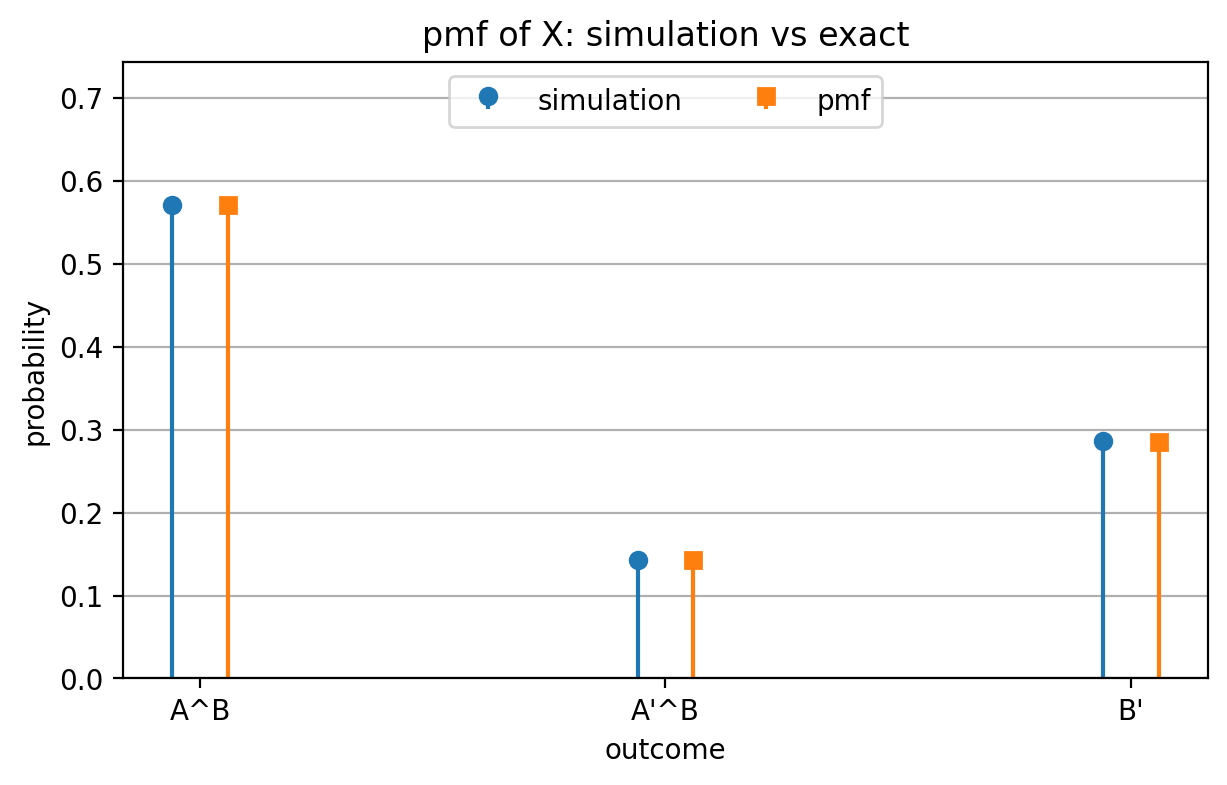
\includegraphics[width=0.8\linewidth]{figs/c12_q17.png}
	\caption{Stem plot of the simulated relative frequencies and the pmf of $X$}
	\label{fig:CBSE12-q17}
\end{figure}

\item
A coin is tossed and a card is selected at random from a well-shuffled pack of $52$ cards. The probability of getting a head and a face card is
\hfill (12, 2025)
% TODO: add options (A)-(D) from the paper; the answer is option (B)

\solution
Let $X = 1$ if the coin shows a head and $0$ otherwise, and $Y = 1$ if the card is a face card and $0$ otherwise. There are $12$ face cards among $52$, so
\begin{table}[H]
	\centering
	\begin{tabular}{|c|c|c|}
		\hline
		$x$ & $0$ & $1$ \\ \hline
		$p_X\brak{x}$ & $\frac{1}{2}$ & $\frac{1}{2}$ \\ \hline
		$p_Y\brak{x}$ & $\frac{40}{52} = \frac{10}{13}$ & $\frac{12}{52} = \frac{3}{13}$ \\ \hline
	\end{tabular}
	\caption{pmfs of $X$ (coin) and $Y$ (card)}
	\label{tab:CBSE12-q18}
\end{table}
The coin and the card are independent, so the joint pmf is the product $p_{XY}\brak{x,y} = p_X\brak{x}p_Y\brak{y}$. A head and a face card is the outcome $\brak{X,Y} = \brak{1,1}$:
\begin{align}
	p_{XY}\brak{1,1} = p_X\brak{1}\,p_Y\brak{1} = \frac{1}{2}\cdot\frac{3}{13} = \frac{3}{26} \quad \brak{\text{Option B}}
\end{align}
The following program simulates $10^6$ tosses and draws and compares the relative frequency with this value
\begin{lstlisting}[frame=single, basicstyle=\rmfamily, escapeinside={(*@}{@*)}]
(*@\makebox[\dimexpr\linewidth-2\fboxsep-2\fboxrule\relax][c]{12/codes/18.c}@*)
\end{lstlisting}
The following code makes a stem plot of the simulated relative frequencies and the pmf, see \figref{fig:CBSE12-q18}.
\begin{lstlisting}[frame=single, basicstyle=\rmfamily, escapeinside={(*@}{@*)}]
(*@\makebox[\dimexpr\linewidth-2\fboxsep-2\fboxrule\relax][c]{12/codes/18plot.py}@*)
\end{lstlisting}
\begin{figure}[H]
	\centering
	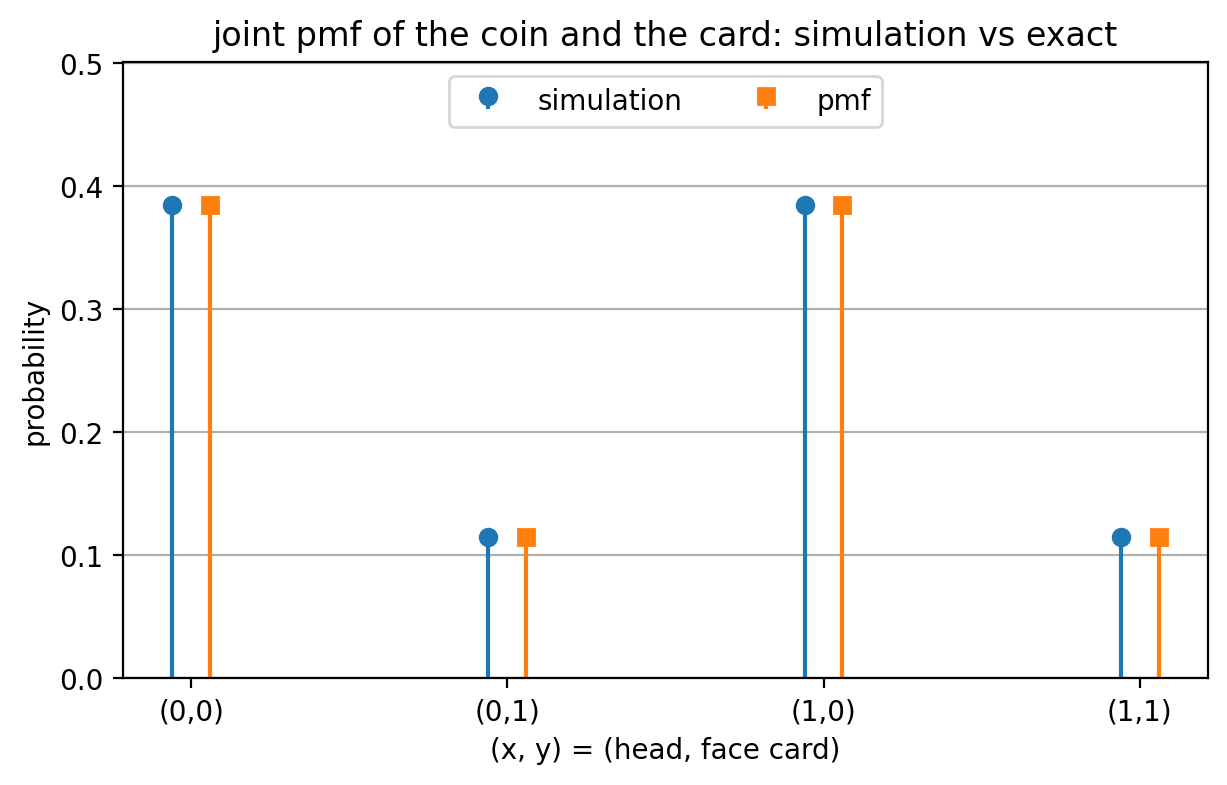
\includegraphics[width=0.8\linewidth]{figs/c12_q18.png}
	\caption{Stem plot of the simulated relative frequencies and the joint pmf of the coin and the card}
	\label{fig:CBSE12-q18}
\end{figure}

\item
If $\vec{A} = \myvec{2 & 3 \\ -1 & 2}$, show that $\vec{A}^2 - 4\vec{A} + 7\vec{I} = \vec{0}$.
\hfill (12, 2025)

\solution
The trace and determinant are
\begin{align}
	\text{tr}\brak{\vec{A}} = 2 + 2 = 4, \qquad \abs{\vec{A}} = 2\brak{2} - 3\brak{-1} = 7
\end{align}
The characteristic polynomial of a $2\times2$ matrix is $\lambda^2 - \text{tr}\brak{\vec{A}}\lambda + \abs{\vec{A}}$, so
\begin{align}
	\lambda^2 - 4\lambda + 7 = 0 \implies \lambda = \frac{4 \pm \sqrt{16-28}}{2} = 2 \pm i\sqrt{3}
\end{align}
The eigenvalues sum to $4$ (the trace) and multiply to $7$ (the determinant). By the Cayley--Hamilton theorem, $\vec{A}$ satisfies its own characteristic equation:
\begin{align}
	\vec{A}^2 - 4\vec{A} + 7\vec{I} = \vec{0}
\end{align}
Direct verification: $\vec{A}^2 = \myvec{1 & 12 \\ -4 & 1}$, $4\vec{A} = \myvec{8 & 12 \\ -4 & 8}$, $7\vec{I} = \myvec{7 & 0 \\ 0 & 7}$, so
\begin{align}
	\vec{A}^2 - 4\vec{A} + 7\vec{I} = \myvec{1-8+7 & 12-12 \\ -4+4 & 1-8+7} = \myvec{0 & 0 \\ 0 & 0}
\end{align}
The following code verifies the solution
\begin{lstlisting}[frame=single, basicstyle=\rmfamily, escapeinside={(*@}{@*)}]
(*@\makebox[\dimexpr\linewidth-2\fboxsep-2\fboxrule\relax][c]{12/codes/22.py}@*)
\end{lstlisting}

\item
Maximise $Z = 5x + 4y$ subject to $3x + y \le 6$, $x \le 1$, $x \ge 0$, $y \ge 0$.
\hfill (12, 2025)

\solution
\textbf{Step 1: the feasible region is convex.} Each constraint is a half-plane $\vec{a}^{\top}\vec{x} \le c$, and a half-plane is a convex set: if $\vec{u}$ and $\vec{w}$ satisfy it, then for $0 \le t \le 1$,
\begin{align}
	\vec{a}^{\top}\brak{t\vec{u} + \brak{1-t}\vec{w}} = t\,\vec{a}^{\top}\vec{u} + \brak{1-t}\vec{a}^{\top}\vec{w} \le c
\end{align}
The feasible region is the intersection of the half-planes given by the constraints, and an intersection of convex sets is convex. So the feasible region is convex.

\textbf{Step 2: graph and corner points.} For a linear objective over a convex feasible region, the optimum (maximum or minimum) lies at a corner point of the region. Plot the boundary lines $3x + y = 6$, $x = 1$, $x = 0$ and $y = 0$ (see \figref{fig:CBSE12-q24}). The corner points are the intersections of pairs of boundary lines that satisfy all the constraints,
\begin{align}
	\brak{0,0},\ \brak{1,0},\ \brak{1,3},\ \brak{0,6}
\end{align}
\begin{table}[H]
	\centering
	\begin{tabular}{|c|c|}
		\hline
		Corner point $\brak{x,y}$ & $Z = 5x + 4y$ \\ \hline
		$\brak{0,0}$ & $0$ \\ \hline
		$\brak{1,0}$ & $5$ \\ \hline
		$\brak{1,3}$ & $17$ \\ \hline
		$\brak{0,6}$ & $24$ \\ \hline
	\end{tabular}
	\caption{Value of $Z$ at the corner points}
	\label{tab:CBSE12-q24}
\end{table}

\textbf{Step 3: optimise with \texttt{cvxpy}.} Since the problem is convex, \texttt{cvxpy} finds the optimum for us. With the variables \texttt{x}, \texttt{y}, the constraints \texttt{[3*x + y <= 6, x <= 1, x >= 0, y >= 0]} and
\begin{lstlisting}[frame=single, basicstyle=\ttfamily\small]
objective = cp.Maximize(5*x + 4*y)
problem = cp.Problem(objective, constraints)
problem.solve()
\end{lstlisting}
the solver returns the same optimum as the corner points,
\begin{align}
	Z_{\max} = 24 \text{ at } \brak{x,y} = \brak{0,6}
\end{align}
The following code checks the convexity, finds the corner points and solves the problem with \texttt{cvxpy}
\begin{lstlisting}[frame=single, basicstyle=\rmfamily, escapeinside={(*@}{@*)}]
(*@\makebox[\dimexpr\linewidth-2\fboxsep-2\fboxrule\relax][c]{12/codes/24.py}@*)
\end{lstlisting}
The following code generates \figref{fig:CBSE12-q24}.
\begin{lstlisting}[frame=single, basicstyle=\rmfamily, escapeinside={(*@}{@*)}]
(*@\makebox[\dimexpr\linewidth-2\fboxsep-2\fboxrule\relax][c]{12/codes/24plot.py}@*)
\end{lstlisting}
\begin{figure}[H]
	\centering
	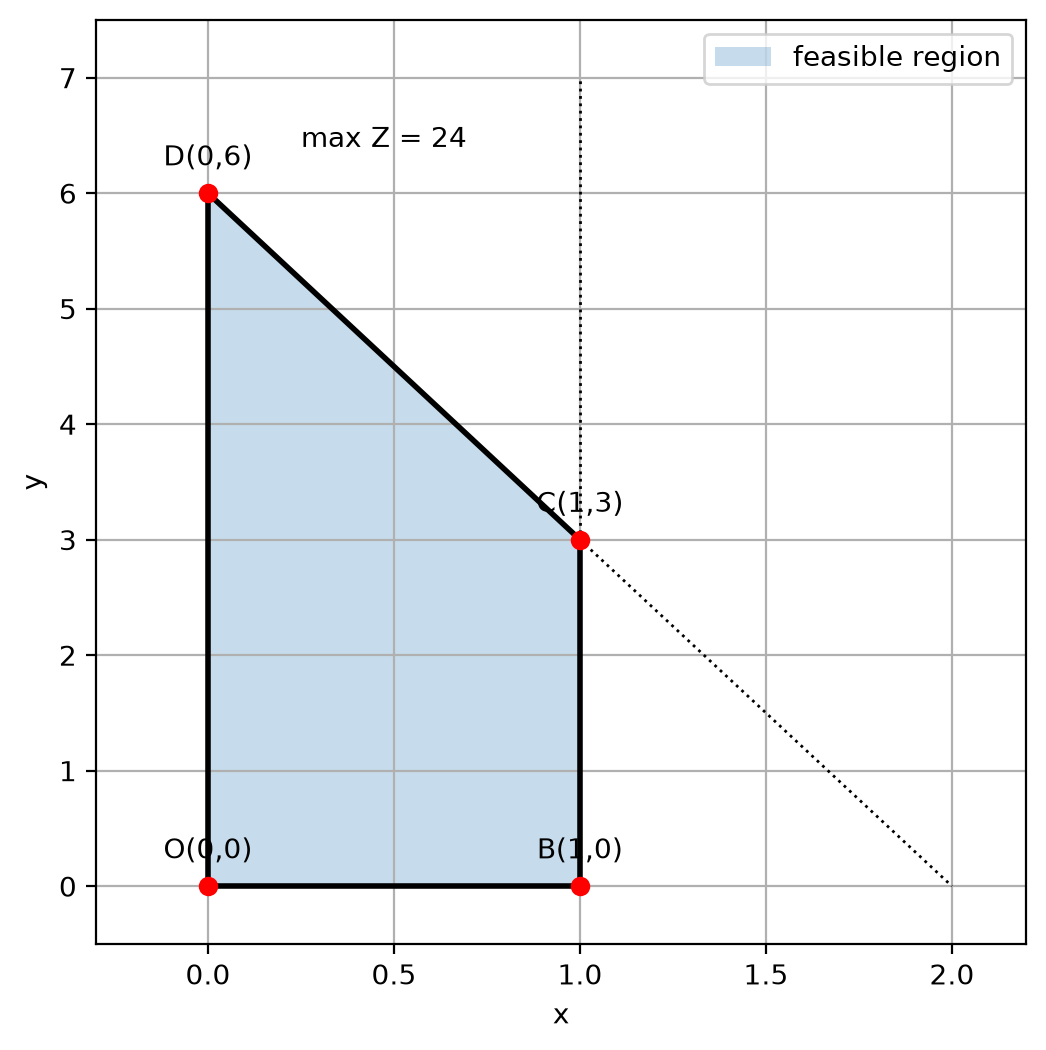
\includegraphics[width=0.5\linewidth]{figs/c12_q24.png}
	\caption{Feasible region and corner points}
	\label{fig:CBSE12-q24}
\end{figure}

\item
A box contains $10$ blocks: two marked $0$, three marked $1$, four marked $2$ and one marked $3$. A block is drawn at random. Find the probability distribution of the number $X$ on the block and its mean.
\hfill (12, 2025)

\solution
Each block is equally likely, so
\begin{align}
	\pr{X=x} = \frac{\text{number of blocks marked } x}{10}
\end{align}
and the pmf is
\begin{table}[H]
	\centering
	\begin{tabular}{|c|c|c|c|c|}
		\hline
		$x$ & $0$ & $1$ & $2$ & $3$ \\ \hline
		$\pr{X=x}$ & $\frac{2}{10}$ & $\frac{3}{10}$ & $\frac{4}{10}$ & $\frac{1}{10}$ \\ \hline
	\end{tabular}
	\caption{Probability mass function of $X$}
	\label{tab:CBSE12-q25}
\end{table}
The probabilities sum to $1$. The mean of $X$ is
\begin{align}
	E\sbrak{X} &= \sum_{x} x\,\pr{X=x} = 0\brak{\frac{2}{10}} + 1\brak{\frac{3}{10}} + 2\brak{\frac{4}{10}} + 3\brak{\frac{1}{10}}
	\\
	&= \frac{14}{10} = 1.4
\end{align}
The following program simulates $10^6$ draws of a block and compares the relative frequencies and the mean with the pmf
\begin{lstlisting}[frame=single, basicstyle=\rmfamily, escapeinside={(*@}{@*)}]
(*@\makebox[\dimexpr\linewidth-2\fboxsep-2\fboxrule\relax][c]{12/codes/25.c}@*)
\end{lstlisting}
The following code makes a stem plot of the simulated relative frequencies and the pmf, see \figref{fig:CBSE12-q25}.
\begin{lstlisting}[frame=single, basicstyle=\rmfamily, escapeinside={(*@}{@*)}]
(*@\makebox[\dimexpr\linewidth-2\fboxsep-2\fboxrule\relax][c]{12/codes/25plot.py}@*)
\end{lstlisting}
\begin{figure}[H]
	\centering
	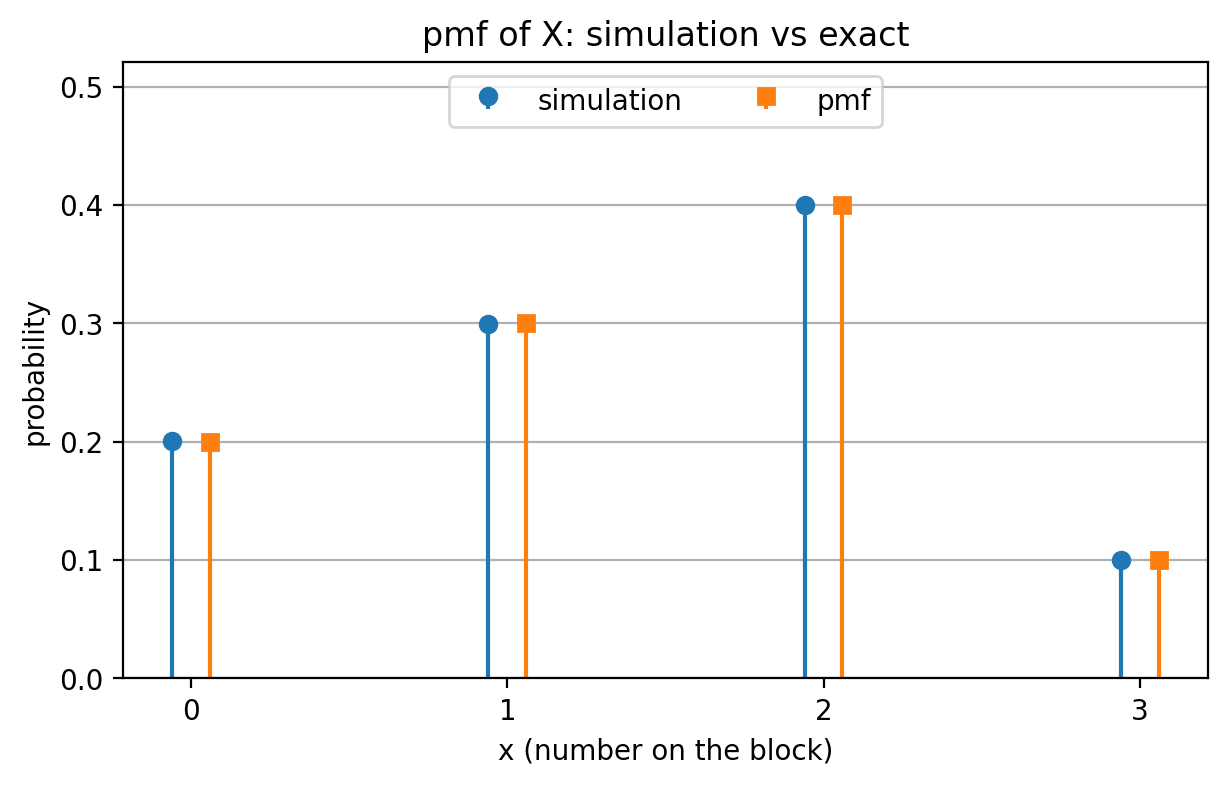
\includegraphics[width=0.8\linewidth]{figs/c12_q25.png}
	\caption{Stem plot of the simulated relative frequencies and the pmf of $X$}
	\label{fig:CBSE12-q25}
\end{figure}

\item
Two ants move along the lines $2x + 5y - 1 = 0$ and $3x + 2y - 7 = 0$. Using the matrix method, find the point where their paths meet.
\hfill (12, 2025)

\solution
In matrix form $\vec{A}\vec{x} = \vec{b}$ with the augmented matrix $\myvec{\vec{A} & \vec{b}}$, Gaussian elimination gives
\begin{align}
	\myvec{2 & 5 & 1 \\ 3 & 2 & 7}
	&\xleftrightarrow[]{R_1 \leftarrow R_1/2}
	\myvec{1 & \frac{5}{2} & \frac{1}{2} \\ 3 & 2 & 7}
	\\
	&\xleftrightarrow[]{R_2 \leftarrow R_2 - 3R_1}
	\myvec{1 & \frac{5}{2} & \frac{1}{2} \\ 0 & -\frac{11}{2} & \frac{11}{2}}
	\\
	&\xleftrightarrow[]{R_2 \leftarrow -\frac{2}{11}R_2}
	\myvec{1 & \frac{5}{2} & \frac{1}{2} \\ 0 & 1 & -1}
	\\
	&\xleftrightarrow[]{R_1 \leftarrow R_1 - \frac{5}{2}R_2}
	\myvec{1 & 0 & 3 \\ 0 & 1 & -1}
\end{align}
Both $\vec{A}$ and $\myvec{\vec{A} & \vec{b}}$ have rank $2$, equal to the number of unknowns, so the lines meet at exactly one point,
\begin{align}
	\vec{x} = \myvec{x \\ y} = \myvec{3 \\ -1}
\end{align}
Check: $2\brak{3} + 5\brak{-1} = 1$ and $3\brak{3} + 2\brak{-1} = 7$. The paths meet at $\brak{3,-1}$. The following code verifies the solution
\begin{lstlisting}[frame=single, basicstyle=\rmfamily, escapeinside={(*@}{@*)}]
(*@\makebox[\dimexpr\linewidth-2\fboxsep-2\fboxrule\relax][c]{12/codes/27.py}@*)
\end{lstlisting}
The following code generates \figref{fig:CBSE12-q27}.
\begin{lstlisting}[frame=single, basicstyle=\rmfamily, escapeinside={(*@}{@*)}]
(*@\makebox[\dimexpr\linewidth-2\fboxsep-2\fboxrule\relax][c]{12/codes/27plot.py}@*)
\end{lstlisting}
\begin{figure}[H]
	\centering
	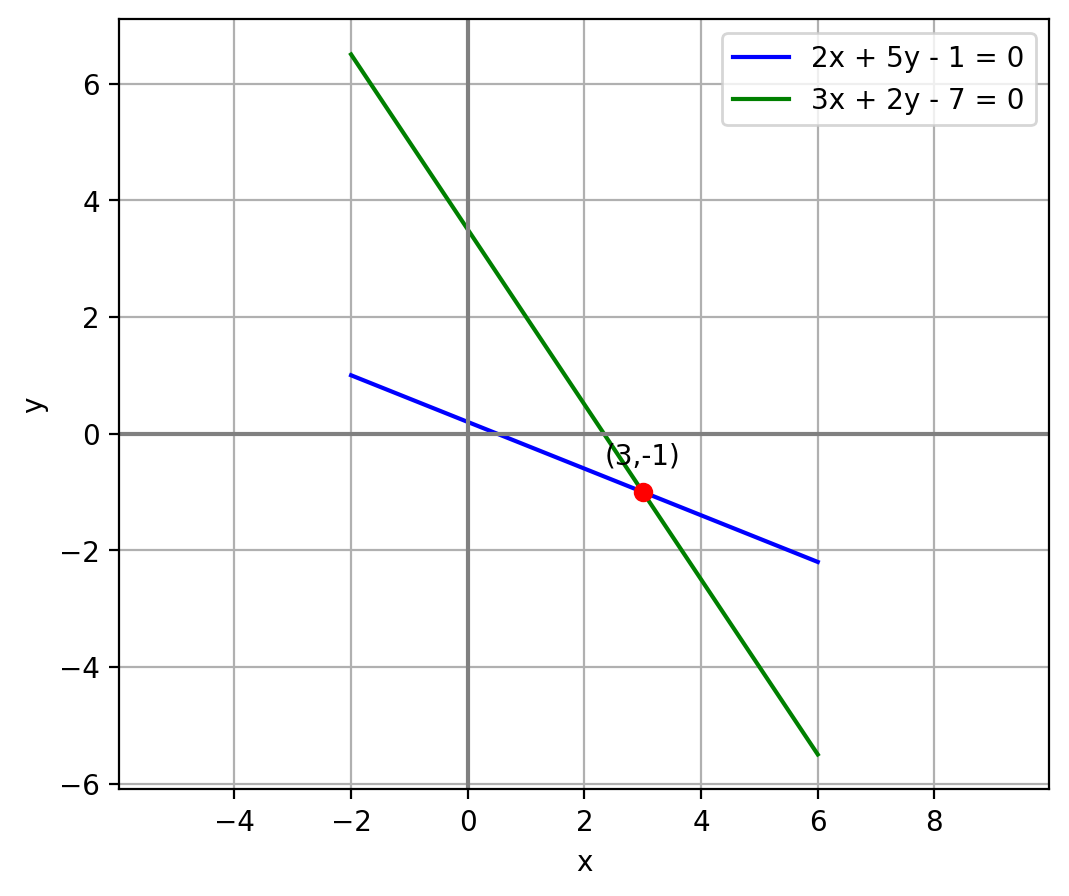
\includegraphics[width=0.6\linewidth]{figs/c12_q27.png}
	\caption{The two paths and their common point $\brak{3,-1}$}
	\label{fig:CBSE12-q27}
\end{figure}

\item
Minimise $Z = 18x + 10y$ subject to $4x + y \ge 20$, $2x + 3y \ge 30$, $x \ge 0$, $y \ge 0$.
\hfill (12, 2025)

\solution
\textbf{Step 1: the feasible region is convex.} Each constraint is a half-plane $\vec{a}^{\top}\vec{x} \le c$, and a half-plane is a convex set: if $\vec{u}$ and $\vec{w}$ satisfy it, then for $0 \le t \le 1$,
\begin{align}
	\vec{a}^{\top}\brak{t\vec{u} + \brak{1-t}\vec{w}} = t\,\vec{a}^{\top}\vec{u} + \brak{1-t}\vec{a}^{\top}\vec{w} \le c
\end{align}
The feasible region is the intersection of the half-planes given by the constraints, and an intersection of convex sets is convex. So the feasible region is convex.

\textbf{Step 2: graph and corner points.} For a linear objective over a convex feasible region, the optimum (maximum or minimum) lies at a corner point of the region. Plot the boundary lines $4x + y = 20$, $2x + 3y = 30$, $x = 0$ and $y = 0$ (see \figref{fig:CBSE12-q30}). The lines $4x + y = 20$ and $2x + 3y = 30$ meet where $y = 20 - 4x$ and $2x + 3\brak{20 - 4x} = 30$, i.e.\ at $\brak{3,8}$. The corner points of the unbounded feasible region are
\begin{align}
	\brak{0,20},\ \brak{3,8},\ \brak{15,0}
\end{align}
\begin{table}[H]
	\centering
	\begin{tabular}{|c|c|}
		\hline
		Corner point $\brak{x,y}$ & $Z = 18x + 10y$ \\ \hline
		$\brak{0,20}$ & $200$ \\ \hline
		$\brak{3,8}$ & $134$ \\ \hline
		$\brak{15,0}$ & $270$ \\ \hline
	\end{tabular}
	\caption{Value of $Z$ at the corner points}
	\label{tab:CBSE12-q30}
\end{table}
Because the region is unbounded, the smallest corner value $134$ is the minimum only if the half-plane $18x + 10y < 134$ has no point in common with the feasible region, which \texttt{cvxpy} confirms below.

\textbf{Step 3: optimise with \texttt{cvxpy}.} Since the problem is convex, \texttt{cvxpy} finds the optimum for us. With the variables \texttt{x}, \texttt{y}, the constraints \texttt{[4*x + y >= 20, 2*x + 3*y >= 30, x >= 0, y >= 0]} and
\begin{lstlisting}[frame=single, basicstyle=\ttfamily\small]
objective = cp.Minimize(18*x + 10*y)
problem = cp.Problem(objective, constraints)
problem.solve()
\end{lstlisting}
the solver returns
\begin{align}
	Z_{\min} = 134 \text{ at } \brak{x,y} = \brak{3,8}
\end{align}
The following code checks the convexity, finds the corner points and solves the problem with \texttt{cvxpy}
\begin{lstlisting}[frame=single, basicstyle=\rmfamily, escapeinside={(*@}{@*)}]
(*@\makebox[\dimexpr\linewidth-2\fboxsep-2\fboxrule\relax][c]{12/codes/30.py}@*)
\end{lstlisting}
The following code generates \figref{fig:CBSE12-q30}.
\begin{lstlisting}[frame=single, basicstyle=\rmfamily, escapeinside={(*@}{@*)}]
(*@\makebox[\dimexpr\linewidth-2\fboxsep-2\fboxrule\relax][c]{12/codes/30plot.py}@*)
\end{lstlisting}
\begin{figure}[H]
	\centering
	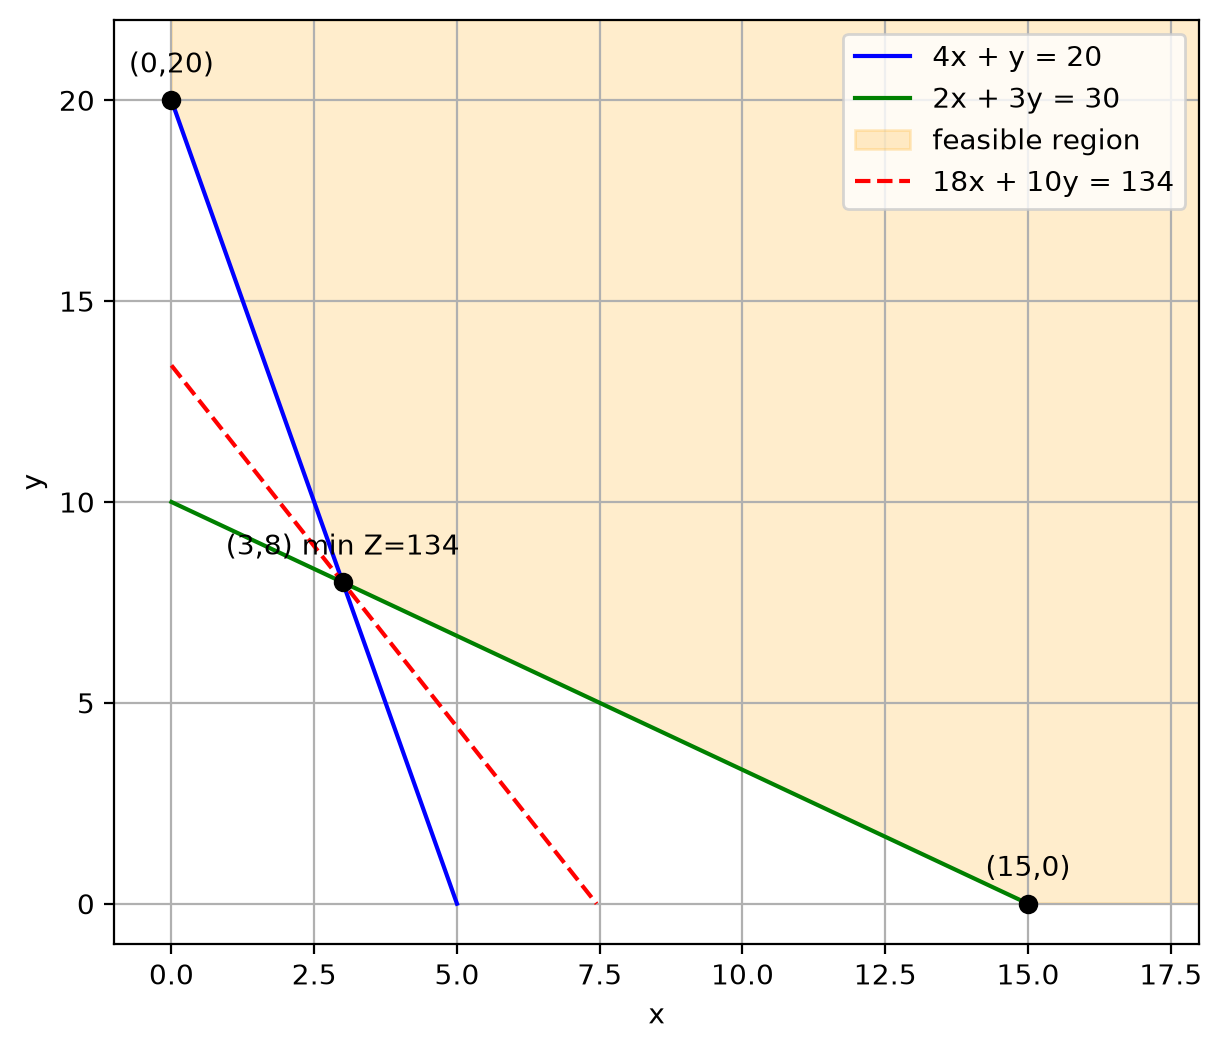
\includegraphics[width=0.6\linewidth]{figs/c12_q30.png}
	\caption{Unbounded feasible region and the line $Z = 134$}
	\label{fig:CBSE12-q30}
\end{figure}

\item
Let $\vec{a} = \hat{i} - \hat{j} + 2\hat{k}$, $\vec{b} = 2\hat{i} - 4\hat{j} + 5\hat{k}$ and $\vec{c} = \lambda\hat{i} - 2\hat{j} - 3\hat{k}$. Find $\lambda$ if the scalar product of $\vec{a}$ with the unit vector along $\vec{b} + \vec{c}$ is $1$.
\hfill (12, 2025)

\solution
\begin{align}
	\vec{b} + \vec{c} = \myvec{\lambda+2 \\ -6 \\ 2}, \qquad \abs{\vec{b}+\vec{c}} = \sqrt{\brak{\lambda+2}^2 + 40}
\end{align}
The scalar product with $\vec{a} = \myvec{1\\-1\\2}$ is
\begin{align}
	\frac{\vec{a}^{\top}\brak{\vec{b}+\vec{c}}}{\abs{\vec{b}+\vec{c}}} = \frac{\lambda + 2 + 6 + 4}{\sqrt{\brak{\lambda+2}^2 + 40}} = \frac{\lambda+12}{\sqrt{\brak{\lambda+2}^2+40}} = 1
\end{align}
Squaring,
\begin{align}
	\brak{\lambda+12}^2 = \brak{\lambda+2}^2 + 40 \implies 20\lambda = -100 \implies \lambda = -5
\end{align}
Check: $\lambda + 12 = 7 > 0$ and $\sqrt{9 + 40} = 7$, so the unsquared equation holds.
The following code verifies the solution
\begin{lstlisting}[frame=single, basicstyle=\rmfamily, escapeinside={(*@}{@*)}]
(*@\makebox[\dimexpr\linewidth-2\fboxsep-2\fboxrule\relax][c]{12/codes/31A.py}@*)
\end{lstlisting}

\item
Find the shortest distance between the lines $\vec{r} = \brak{2\hat{i} - \hat{j} + 3\hat{k}} + \lambda\brak{\hat{i} - 2\hat{j} + 3\hat{k}}$ and $\vec{r} = \brak{\hat{i} + 4\hat{k}} + \mu\brak{3\hat{i} - 6\hat{j} + 9\hat{k}}$.
\hfill (12, 2025)

\solution
The lines are
\begin{align}
	\vec{x} = \vec{A} + \kappa_1\vec{m}_1, \quad \vec{x} = \vec{B} + \kappa_2\vec{m}_2
	\\
	\vec{A} = \myvec{2\\-1\\3},\ \vec{B} = \myvec{1\\0\\4},\ \vec{m}_1 = \myvec{1\\-2\\3},\ \vec{m}_2 = \myvec{3\\-6\\9}
\end{align}
With $\vec{M} = \myvec{\vec{m}_1 & \vec{m}_2}$, row reduction gives
\begin{align}
	\myvec{1 & 3 \\ -2 & -6 \\ 3 & 9}
	\xleftrightarrow[R_3 \leftarrow R_3 - 3R_1]{R_2 \leftarrow R_2 + 2R_1}
	\myvec{1 & 3 \\ 0 & 0 \\ 0 & 0}
\end{align}
so $\text{rank}\brak{\vec{M}} = 1$ and the lines are parallel, with $\vec{m}_2 = 3\vec{m}_1$. The squared distance between a point of each line is
\begin{align}
	\norm{\vec{A} + \kappa_1\vec{m}_1 - \vec{B} - \kappa_2\vec{m}_2}^2 = \norm{\brak{\vec{A}-\vec{B}} + \kappa\vec{m}_1}^2, \quad \kappa = \kappa_1 - 3\kappa_2
\end{align}
which is least when its derivative with respect to $\kappa$ vanishes, i.e.\ for the normal equation
\begin{align}
	\vec{m}_1^{\top}\vec{m}_1\,\kappa = \vec{m}_1^{\top}\brak{\vec{B} - \vec{A}}
	\implies 14\kappa = \myvec{1 & -2 & 3}\myvec{-1\\1\\1} = 0 \implies \kappa = 0
\end{align}
Hence the closest point on the first line is $\vec{A}$ itself and the shortest distance is
\begin{align}
	d = \norm{\vec{A} - \vec{B}} = \norm{\myvec{1\\-1\\-1}} = \sqrt{3}
\end{align}
The following code verifies the solution, including the least squares solution used in matgeo
\begin{lstlisting}[frame=single, basicstyle=\rmfamily, escapeinside={(*@}{@*)}]
(*@\makebox[\dimexpr\linewidth-2\fboxsep-2\fboxrule\relax][c]{12/codes/31B.py}@*)
\end{lstlisting}

\item
Evaluate $\displaystyle\int_0^{\pi} \frac{x\tan x}{\sec x + \tan x}\,dx$.
\hfill (12, 2025)

\solution
Since $\frac{\tan x}{\sec x + \tan x} = \frac{\sin x}{1 + \sin x}$, the integral is $I = \int_0^\pi \frac{x\sin x}{1+\sin x}\,dx$. Using $\int_0^\pi xg\brak{x}\,dx = \frac{\pi}{2}\int_0^\pi g\brak{x}\,dx$ when $g\brak{\pi-x} = g\brak{x}$,
\begin{align}
	I = \frac{\pi}{2}\int_0^\pi \frac{\sin x}{1+\sin x}\,dx = \frac{\pi}{2}\int_0^\pi\brak{1 - \frac{1}{1+\sin x}}dx
\end{align}
Rationalising, $\frac{1}{1+\sin x} = \sec^2 x - \sec x\tan x$, whose antiderivative is $\tan x - \sec x$. Over $\sbrak{0,\pi}$ this gives $\int_0^\pi\frac{dx}{1+\sin x} = 2$ (the point $x = \frac{\pi}{2}$ is handled by taking limits on either side). Hence
\begin{align}
	I = \frac{\pi}{2}\brak{\pi - 2} \approx 1.7932
\end{align}
To evaluate the integral numerically, divide $\sbrak{0,\pi}$ into $N$ strips of width $h = \frac{\pi}{N}$ with nodes $x_n = nh$ and let $g\brak{x} = \frac{x\sin x}{1+\sin x}$. Define the running integral
\begin{align}
	I\sbrak{n} = \int_0^{x_n} g\brak{x}\,dx, \quad I\sbrak{0} = 0
\end{align}
The strip between $x_n$ and $x_{n+1}$ is approximated by a trapezoid with parallel sides $g\brak{x_n}$ and $g\brak{x_{n+1}}$ and width $h$, whose area is $\frac{h}{2}\brak{g\brak{x_n} + g\brak{x_{n+1}}}$. Hence $I$ satisfies the difference equation
\begin{align}
	I\sbrak{n+1} = I\sbrak{n} + \frac{h}{2}\brak{g\brak{x_n} + g\brak{x_{n+1}}}, \quad I\sbrak{0} = 0
\end{align}
and the integral is $I\sbrak{N}$. Summing the equation over $n = 0,\dots,N-1$ gives the trapezoidal rule
\begin{align}
	I\sbrak{N} = \frac{h}{2}\brak{g\brak{x_0} + 2\sum_{n=1}^{N-1}g\brak{x_n} + g\brak{x_N}}
\end{align}
Iterating the difference equation gives $I\sbrak{12} = 1.7754$, $I\sbrak{100} = 1.79295$ and $I\sbrak{1000} = 1.79321$, approaching $1.79321$. The following code verifies the solution
\begin{lstlisting}[frame=single, basicstyle=\rmfamily, escapeinside={(*@}{@*)}]
(*@\makebox[\dimexpr\linewidth-2\fboxsep-2\fboxrule\relax][c]{12/codes/32B.py}@*)
\end{lstlisting}
The following code generates \figref{fig:CBSE12-q32B}.
\begin{lstlisting}[frame=single, basicstyle=\rmfamily, escapeinside={(*@}{@*)}]
(*@\makebox[\dimexpr\linewidth-2\fboxsep-2\fboxrule\relax][c]{12/codes/32Bplot.py}@*)
\end{lstlisting}
\begin{figure}[H]
	\centering
	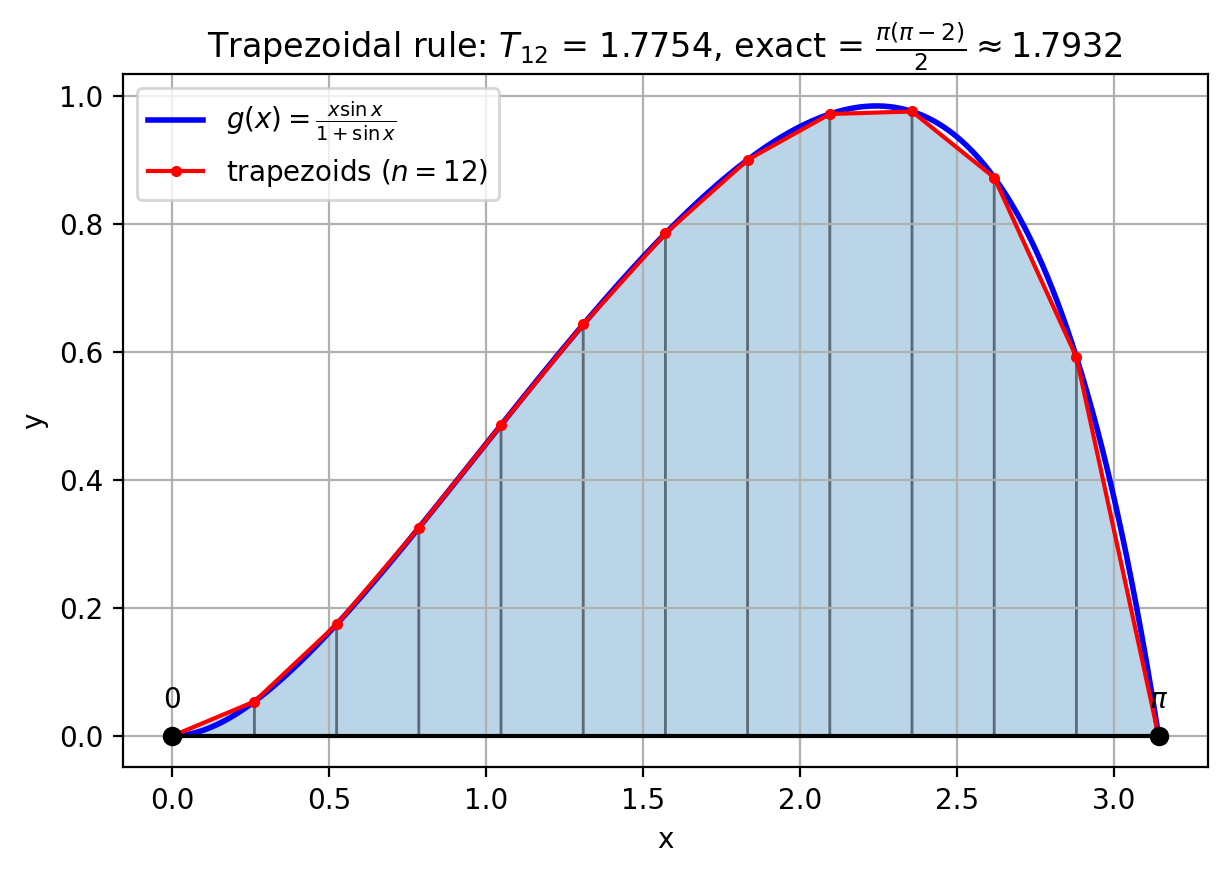
\includegraphics[width=0.6\linewidth]{figs/c12_q32B.png}
	\caption{Trapezoidal rule ($n = 12$) for $\frac{x\sin x}{1+\sin x}$ on $\sbrak{0,\pi}$}
	\label{fig:CBSE12-q32B}
\end{figure}

\item
Solve $\dfrac{dy}{dx} = \cos x - 2y$ using Laplace transforms.
\hfill (12, 2025)

\solution
Rewrite as $y^{\prime} + 2y = \cos x$ and let $Y\brak{s} = \mathcal{L}\cbrak{y}$, $y\brak{0} = y_0$. Since $\mathcal{L}\cbrak{y^{\prime}} = sY - y_0$ and $\mathcal{L}\cbrak{\cos x} = \frac{s}{s^2+1}$,
\begin{align}
	\brak{s+2}Y\brak{s} = y_0 + \frac{s}{s^2+1} \implies Y\brak{s} = \frac{y_0}{s+2} + \frac{s}{\brak{s+2}\brak{s^2+1}}
\end{align}
Partial fractions: $\frac{s}{\brak{s+2}\brak{s^2+1}} = \frac{-\frac{2}{5}}{s+2} + \frac{\frac{2}{5}s + \frac{1}{5}}{s^2+1}$. Using $\mathcal{L}^{-1}\cbrak{\frac{1}{s+2}} = e^{-2x}$, $\mathcal{L}^{-1}\cbrak{\frac{s}{s^2+1}} = \cos x$ and $\mathcal{L}^{-1}\cbrak{\frac{1}{s^2+1}} = \sin x$,
\begin{align}
	y\brak{x} = \brak{y_0 - \frac{2}{5}}e^{-2x} + \frac{2}{5}\cos x + \frac{1}{5}\sin x = Ce^{-2x} + \frac{2\cos x + \sin x}{5}
\end{align}
No initial condition is given, so the constant $C$ is arbitrary. The following code verifies the solution
\begin{lstlisting}[frame=single, basicstyle=\rmfamily, escapeinside={(*@}{@*)}]
(*@\makebox[\dimexpr\linewidth-2\fboxsep-2\fboxrule\relax][c]{12/codes/34.py}@*)
\end{lstlisting}

\item
Find the points on the line $\dfrac{2x+4}{6} = \dfrac{y+1}{2} = \dfrac{-2z+6}{-4}$ at a distance of $3\sqrt{2}$ units from the point $P\brak{1,2,3}$.
\hfill (12, 2025)

\solution
Let the common ratio be $\kappa$. Then $x = 3\kappa - 2$, $y = 2\kappa - 1$, $z = 2\kappa + 3$, which is the parametric form
\begin{align}
	\vec{x} = \vec{A} + \kappa\vec{m}, \quad \vec{A} = \myvec{-2\\-1\\3}, \quad \vec{m} = \myvec{3\\2\\2}
\end{align}
A point of the line is at distance $3\sqrt{2}$ from $\vec{P} = \myvec{1\\2\\3}$ when $\norm{\vec{A} + \kappa\vec{m} - \vec{P}}^2 = 18$. With $\vec{d} = \vec{A} - \vec{P} = \myvec{-3\\-3\\0}$,
\begin{align}
	\brak{\vec{m}^{\top}\vec{m}}\kappa^2 + 2\brak{\vec{m}^{\top}\vec{d}}\kappa + \vec{d}^{\top}\vec{d} = 18
	\implies 17\kappa^2 - 30\kappa + 18 = 18
\end{align}
\begin{align}
	\kappa\brak{17\kappa - 30} = 0 \implies \kappa = 0 \text{ or } \kappa = \frac{30}{17}
\end{align}
The required points are
\begin{align}
	\vec{Q}_1 = \vec{A} = \myvec{-2\\-1\\3}, \qquad \vec{Q}_2 = \vec{A} + \frac{30}{17}\vec{m} = \myvec{\frac{56}{17}\\\frac{43}{17}\\\frac{111}{17}}
\end{align}
The following code verifies the solution
\begin{lstlisting}[frame=single, basicstyle=\rmfamily, escapeinside={(*@}{@*)}]
(*@\makebox[\dimexpr\linewidth-2\fboxsep-2\fboxrule\relax][c]{12/codes/35A.py}@*)
\end{lstlisting}
The following code generates \figref{fig:CBSE12-q35A}.
\begin{lstlisting}[frame=single, basicstyle=\rmfamily, escapeinside={(*@}{@*)}]
(*@\makebox[\dimexpr\linewidth-2\fboxsep-2\fboxrule\relax][c]{12/codes/35Aplot.py}@*)
\end{lstlisting}
\begin{figure}[H]
	\centering
	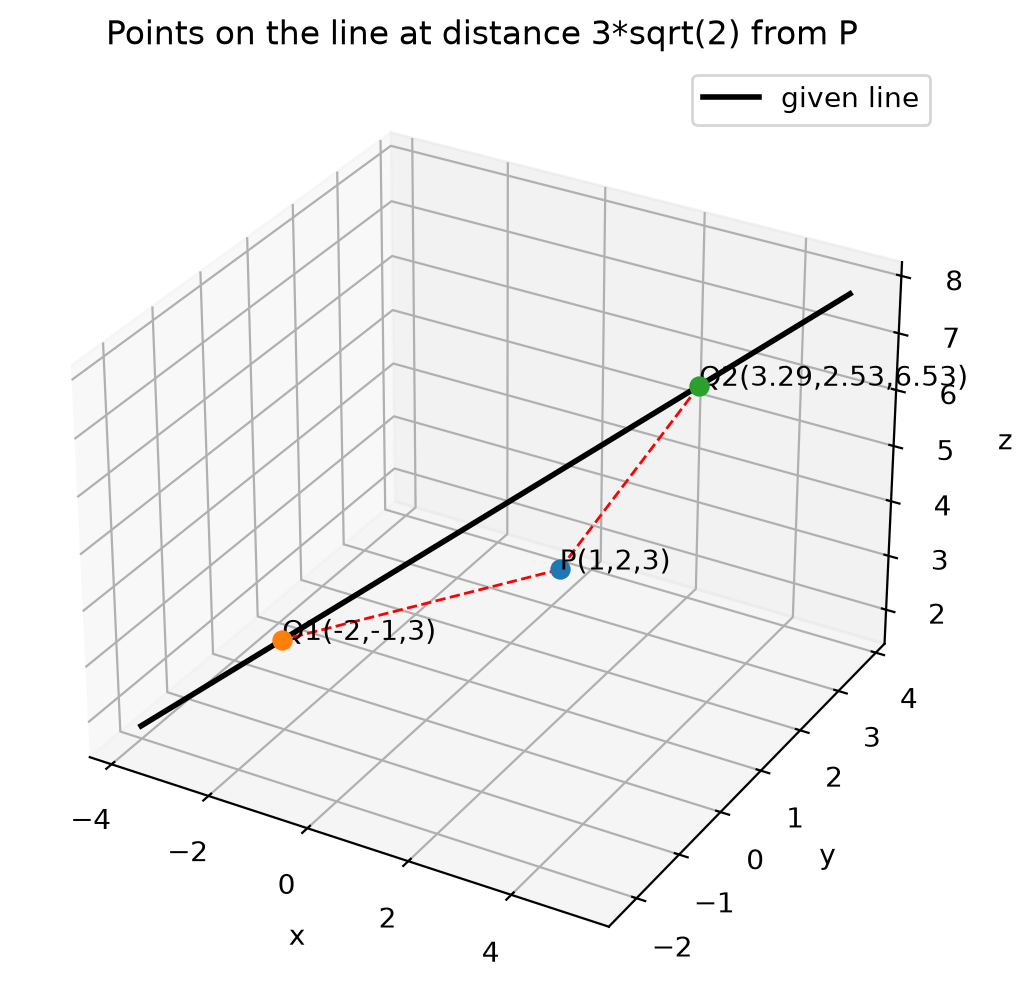
\includegraphics[width=0.6\linewidth]{figs/c12_q35A.png}
	\caption{Points $Q_1$, $Q_2$ on the line at distance $3\sqrt{2}$ from $P$}
	\label{fig:CBSE12-q35A}
\end{figure}

\item
Find the image of the point $P\brak{-1,5,2}$ in the line $\dfrac{2x-4}{2} = \dfrac{y}{2} = \dfrac{2-z}{3}$, and the length $PP^{\prime}$.
\hfill (12, 2025)

\solution
Let the common ratio be $\kappa$. Then $x = \kappa + 2$, $y = 2\kappa$, $z = 2 - 3\kappa$, which is the parametric form
\begin{align}
	\vec{x} = \vec{A} + \kappa\vec{m}, \quad \vec{A} = \myvec{2\\0\\2}, \quad \vec{m} = \myvec{1\\2\\-3}
\end{align}
The foot of the perpendicular $\vec{H} = \vec{A} + \kappa_0\vec{m}$ from $\vec{P} = \myvec{-1\\5\\2}$ satisfies $\vec{m}^{\top}\brak{\vec{H} - \vec{P}} = 0$, so
\begin{align}
	\kappa_0 = \frac{\vec{m}^{\top}\brak{\vec{P}-\vec{A}}}{\vec{m}^{\top}\vec{m}} = \frac{\myvec{1&2&-3}\myvec{-3\\5\\0}}{14} = \frac{7}{14} = \frac{1}{2}
	\implies \vec{H} = \myvec{\frac{5}{2}\\1\\\frac{1}{2}}
\end{align}
Since $\vec{H}$ is the mid-point of $\vec{P}$ and its image $\vec{P}^{\prime}$,
\begin{align}
	\vec{P}^{\prime} = 2\vec{H} - \vec{P} = \myvec{5\\2\\1} - \myvec{-1\\5\\2} = \myvec{6\\-3\\-1}
\end{align}
\begin{align}
	PP^{\prime} = \norm{\vec{P}^{\prime} - \vec{P}} = \norm{\myvec{7\\-8\\-3}} = \sqrt{49 + 64 + 9} = \sqrt{122}
\end{align}
The following code verifies the solution
\begin{lstlisting}[frame=single, basicstyle=\rmfamily, escapeinside={(*@}{@*)}]
(*@\makebox[\dimexpr\linewidth-2\fboxsep-2\fboxrule\relax][c]{12/codes/35B.py}@*)
\end{lstlisting}
The following code generates \figref{fig:CBSE12-q35B}.
\begin{lstlisting}[frame=single, basicstyle=\rmfamily, escapeinside={(*@}{@*)}]
(*@\makebox[\dimexpr\linewidth-2\fboxsep-2\fboxrule\relax][c]{12/codes/35Bplot.py}@*)
\end{lstlisting}
\begin{figure}[H]
	\centering
	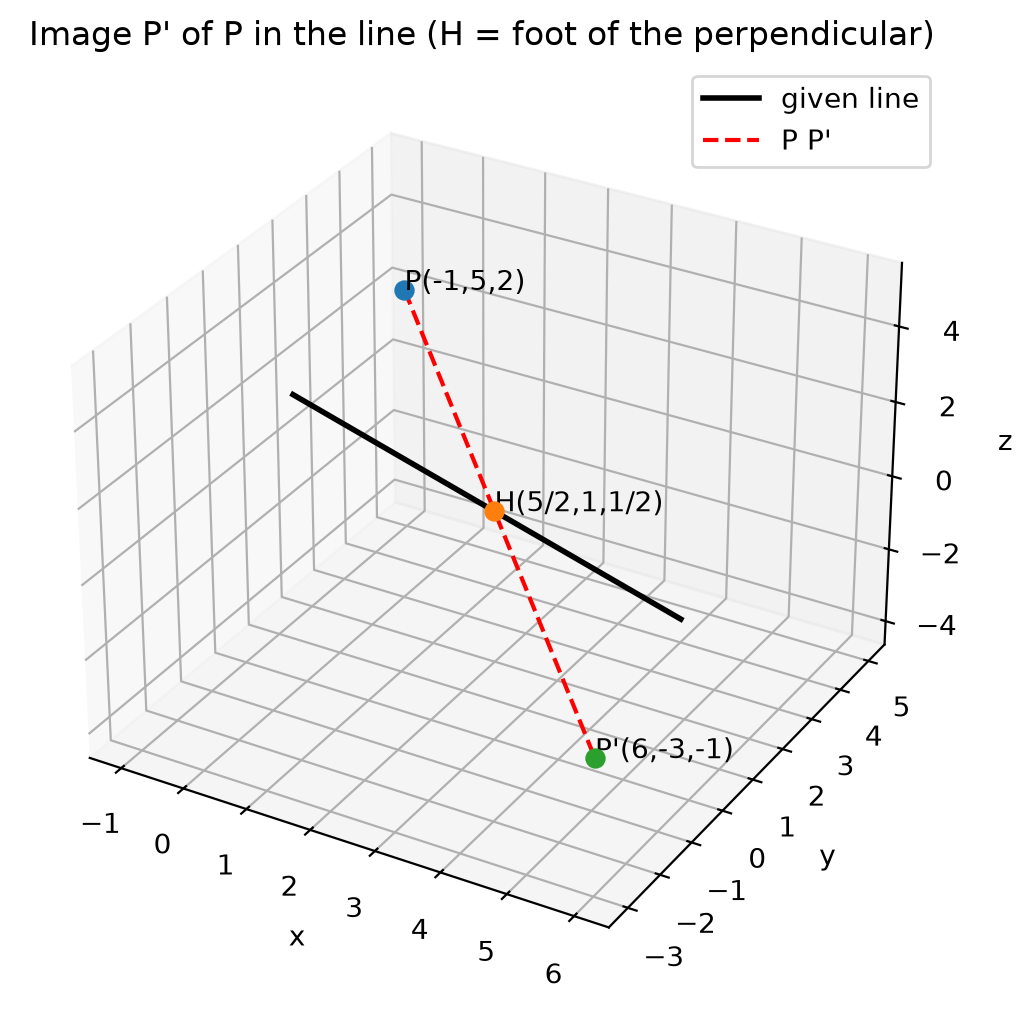
\includegraphics[width=0.6\linewidth]{figs/c12_q35B.png}
	\caption{Point $P$, its image $P^{\prime}$ and the foot $H$}
	\label{fig:CBSE12-q35B}
\end{figure}

\item
\textbf{Case study (health survey).} Of $1000$ people, $700$ have good health ($A_1$), $200$ average health ($A_2$) and $100$ poor health ($A_3$). The probabilities of contracting the disease $D$ are $\pr{D\mid A_1} = 0.25$, $\pr{D\mid A_2} = 0.35$ and $\pr{D\mid A_3} = 0.50$. (i) Find the probability that a randomly selected person has contracted the disease. (ii) Find the probability that a person who has not contracted the disease belongs to category $A_1$.
\hfill (12, 2025)

\solution
Let $X = 1, 2, 3$ denote the category $A_X$. The pmf of $X$ and the conditional probabilities of the disease are
\begin{table}[H]
	\centering
	\begin{tabular}{|c|c|c|c|}
		\hline
		$x$ & $1$ & $2$ & $3$ \\ \hline
		$p_X\brak{x} = \pr{A_x}$ & $0.70$ & $0.20$ & $0.10$ \\ \hline
		$\pr{D\mid A_x}$ & $0.25$ & $0.35$ & $0.50$ \\ \hline
		$\pr{D^{\prime}\mid A_x} = 1 - \pr{D\mid A_x}$ & $0.75$ & $0.65$ & $0.50$ \\ \hline
	\end{tabular}
	\caption{pmf of the category and conditional probabilities}
	\label{tab:CBSE12-q38}
\end{table}
The joint pmf follows from $\pr{A_x\cap D} = p_X\brak{x}\pr{D\mid A_x}$:
\begin{table}[H]
	\centering
	\begin{tabular}{|c|c|c|c|}
		\hline
		$x$ & $1$ & $2$ & $3$ \\ \hline
		$\pr{A_x\cap D}$ & $0.175$ & $0.070$ & $0.050$ \\ \hline
		$\pr{A_x\cap D^{\prime}}$ & $0.525$ & $0.130$ & $0.050$ \\ \hline
	\end{tabular}
	\caption{Joint pmf of the category and the disease}
	\label{tab:CBSE12-q38-joint}
\end{table}
\textbf{(i)} Summing over the categories (law of total probability),
\begin{align}
	\pr{D} = 0.175 + 0.070 + 0.050 = 0.295
\end{align}
\textbf{(ii)} Similarly $\pr{D^{\prime}} = 0.525 + 0.130 + 0.050 = 0.705 = 1 - 0.295$. By Bayes' theorem,
\begin{align}
	\pr{A_1\mid D^{\prime}} = \frac{\pr{A_1\cap D^{\prime}}}{\pr{D^{\prime}}} = \frac{0.525}{0.705} = \frac{35}{47} \approx 0.7447
\end{align}
The following program simulates the category and the disease of $10^6$ people and compares the relative frequencies with these values
\begin{lstlisting}[frame=single, basicstyle=\rmfamily, escapeinside={(*@}{@*)}]
(*@\makebox[\dimexpr\linewidth-2\fboxsep-2\fboxrule\relax][c]{12/codes/38.c}@*)
\end{lstlisting}
The following code makes a stem plot of the simulated relative frequencies and the pmf, see \figref{fig:CBSE12-q38}.
\begin{lstlisting}[frame=single, basicstyle=\rmfamily, escapeinside={(*@}{@*)}]
(*@\makebox[\dimexpr\linewidth-2\fboxsep-2\fboxrule\relax][c]{12/codes/38plot.py}@*)
\end{lstlisting}
\begin{figure}[H]
	\centering
	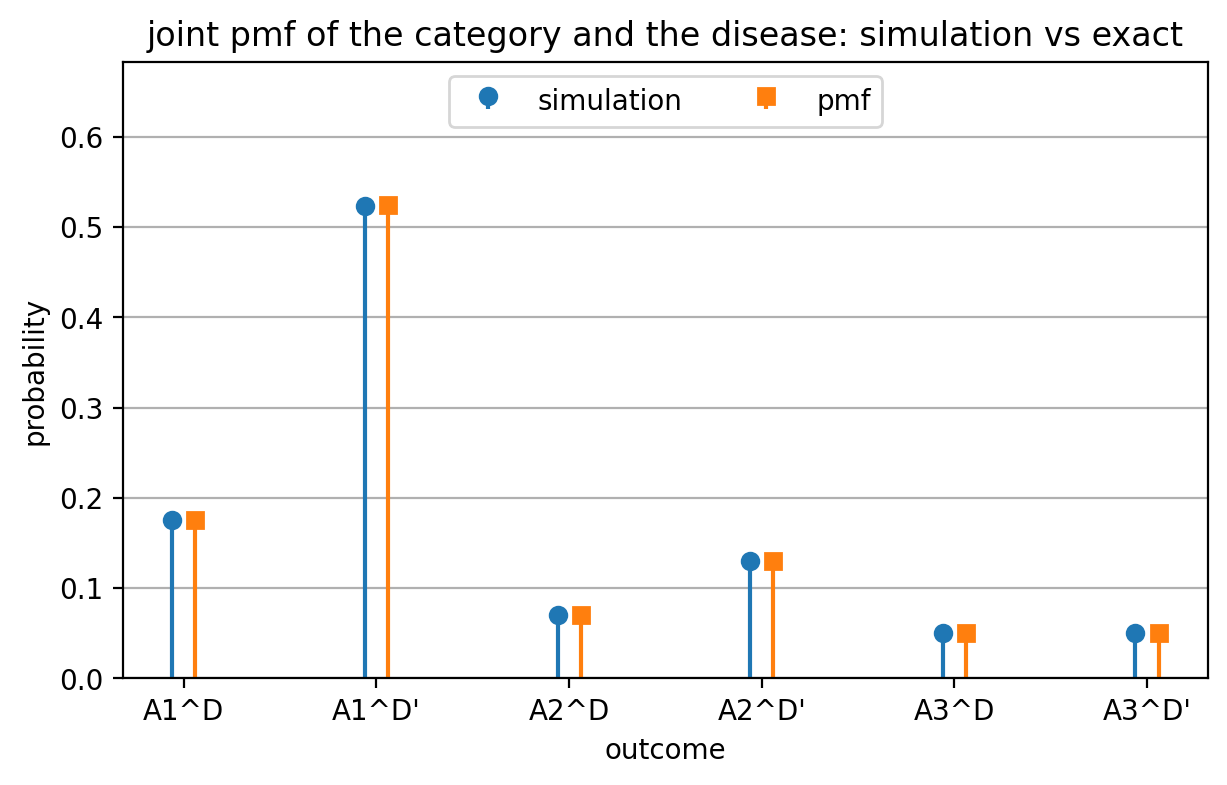
\includegraphics[width=0.8\linewidth]{figs/c12_q38.png}
	\caption{Stem plot of the simulated relative frequencies and the joint pmf of the category and the disease}
	\label{fig:CBSE12-q38}
\end{figure}

\end{enumerate}
